\label{zr}

\citet{Zipf1949} famously observes the linear relationship between log rank $r$ and log word frequency $f(r)$ in several linguistic samples. This is generalized below:

\begin{unlabeledexample} 
$\displaystyle f(C, \alpha) = \frac{C}{r^\alpha}$ 
\end{unlabeledexample} 

\noindent 
$C$ is a constant, sensitive to sample size. \citeauthor{Zipf1949} assumes a 1-to-1 relationship, implying $\alpha = -1$, but it is possible to compute an optimal estimate for this parameter by taking the logarithm of both sides of the equation and solving for values of $C$ and $\alpha$ that minimize the error term $\epsilon$; this can be done efficiently with linear regression:

\begin{unlabeledexample} 
$\displaystyle \textrm{log}~f(r) \sim \textrm{log}~C + \alpha~\textrm{log}~r + \epsilon$  
\end{unlabeledexample}

\citet{Good1953} notes that sparse distributions exhibit quantization at low frequencies, resulting in an artificially long flat right tail imposing an upward bias on estimates of $\alpha$. \citet[][29]{Church1991} propose a transform which eliminates this quantization. The vectors $r, n$ are defined so such that $n_i$ is the number of types which occur at frequency $r_i$ (that is, $n$ is a vector of frequencies of individual type frequencies). $Z$ contains the elements of $n$ by normalized by the points to the left and right.

\begin{unlabeledexample}
$\displaystyle Z_i = \frac{2 n_i}{r_{i + 1} - r_{i - 1}}$
\end{unlabeledexample}

\noindent \citeauthor{Church1991} do not define this transform for the lowest and highest points (i.e., when $i = 1$ or $N$), but a natural extension of their definition is to scale the endpoints according to the next intermost point, as defined below.

\begin{unlabeledexample}
$\displaystyle Z_1 = \frac{n_1}{r_2 - r_1}$
\end{unlabeledexample}

\begin{unlabeledexample}
$\displaystyle Z_N = \frac{n_N}{r_N - r_{N - 1}}$
\end{unlabeledexample}

\noindent The effect of applying this transform to sparse frequency data is shown in Figure \ref{subtlex}.

\begin{figure}
\centering
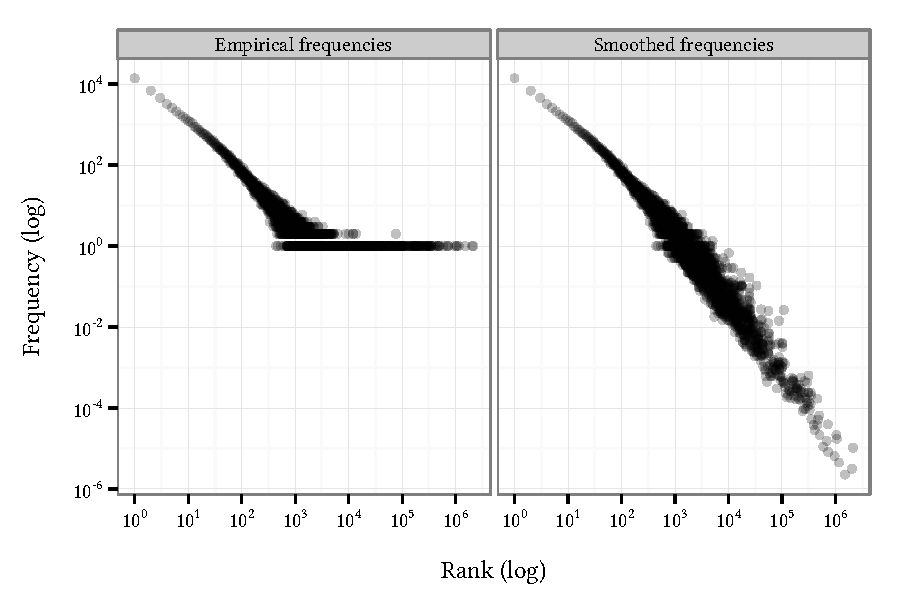
\includegraphics{zr.pdf}
\caption{The left panel shows the empirical word frequencies from the SUBTLEX-US frequency norms \citep{Brysbaert2009}. The right panel shows the same frequencies smoothed with the $Z_r$ transform.}
\label{subtlex}
\end{figure}
